

\section{Overview} 
This chapter discusses the multiple knapsack problem (MKP) and the assignment problem, as well as several hybridizations of exact and heuristic methods to solve each.  The traditional knapsack problem (KP) is a combinatorial optimization problem concerned with finding the optimal combination of \textit{j} out of $n$ items with values $p_j$ and weights $w_j$, to fill a ``knapsack" to maximize value without busting the knapsack capacity constraint, $c$ \cite{knapsackProblems}. 
\begin{align}
\begin{cases}
\max &\sum_{j=1}^n p_jx_j\\
\text{subject to} &\sum_{j=1}^n w_jx_j\leq c\\
&x_j \in \{0,1\} \text{,}	\hspace{5mm}\text{j=1,...,n}
\end{cases}
\end{align}

It is one of Karp's NP-Complete problems \cite{Karp2010ReducibilityProblems}. Approaches that compute optimal solutions for the KP are the use of dynamic programming and the branch and bound method. Both approaches can be time and memory consuming for trivial instances of the KP and are not practical.         
Approximation schemes solve the problem to optimality or close to optimality while saving time and memory.
Recent research by Haddar \textit{et al.} \cite{Haddar2016} uses an evolutionary computation technique, the Quantum Particle Swarm Optimization (QPSO), with a local search method in order to solve the KP. 
The KP has many real life applications other than bag packing, such as cutting stock, capital budgeting, and cryptography \cite{Wilbaut2008}.  Kosuch and Lisser \cite{Kosuch2011OnProblems} studied a particular instance of a stochastic knapsack where items of unknown weight are assigned to knapsacks in a first stage and can be taken out or added to the knapsack after a second stage, when the actual weights become known. They proved that when searching for good lower bounds, one can replace an exhaustive branch-and-bound framework
by a heuristic.  Perry and Hartman \cite{Perry2009} modeled a case of a stochastic dynamic knapsack, where items arrive according to a stochastic process and stay in the knapsack for a number of time periods before exiting. Ross and Tsang \cite{Ross1989} applied the concept of a stochastic dynamic knapsack to bandwidth allocations of communications switching network to randomly arriving calls of random length.        

%A special case of a KP, known as a multidimensional knapsack problem, seeks to find a subset of items that maximizes a linear objective function while satisfying a set of linear capacity constraints.

\section{Multiple Knapsack}
The multiple knapsack problem is an extension of the KP problem where there are \textit{n} items and \textit{m} knapsacks $(m\leq n)$. When $m=1$, a MKP reduces to the traditional KP problem \cite{MKPChapter}. 

\begin{align}
\begin{cases}
\max 				&\sum_{i=1}^m\sum_{j=1}^n p_jx_{ij} \\
\text{subject to}   &\sum_{j=1}^n w_jx_{ij}\leq c_i \text{,}	 \hspace{5mm}\text{i=1,...,m}\\
					&\sum_{i=1}^m x_{ij}\leq 1 		\text{,} 	 \hspace{5mm}\text{j=1,...,n}\\
					&x_{ij} \in \{0,1\} 				\text{,} \hspace{5mm}\text{i=1,...,m} \text{,}	 \hspace{5mm}\text{j=1,...,n}
\end{cases}
\end{align}

The first MKP was published by Eilon and Christofides \cite{EilonChristofides1971} in 1971 as a loading problem ``defined as the allocation of items with known magnitude to boxes with constrained capacity so as to minimize the number of boxes required" \cite{EilonChristofides1971}.  The recommended solutions were to use a zero-one programming model and a heuristic.  The heuristic involved a cycle of scanning for items to precisely fill boxes and performed well compared to the zero-one programming method, finding the optimal solution to 48 out of 50 problems in significantly less computing time in comparison.  More recently, Lai \textit{et al.} \cite{Lai2018} innovated an effective hybrid evolutionary algorithm using a solution-based tabu search for solving the MKP. As of 2017, their algorithm reproduced the best known results for the vast majority of instances tested and established new best known solutions, or improved lower bounds, for four hard instances.  To solve a dynamic, stochastic MKP, Perry and Hartman \cite{Perry2009} presented a stochastic dynamic program (SDP) recursion. Their approximation approach utilizes simulation and deterministic dynamic programming  to allow for the solution of longer horizon problems and ensure good time zero decisions. 
Solutions to the MKP can aid in more than answering physical allocation issues; Simon \textit{et al.} \cite{Simon2017} applied the MKP to assess the different factors that impact Marine self-sufficiency.

\section{Multidimensional Knapsack}
Differing from the multiple knapsack, the multidimensional knapsack problem is an extension of the KP problem where there are multiple resource constraints or a constraint with a multidimensional attribute \cite{knapsackProblems}. 
\begin{align}
\begin{cases}
\max &\sum_{j=1}^n p_jx_j\\
\text{subject to} &\sum_{j=1}^n w_{ij}x_j\leq c_i \hspace{5mm}\text{i=1,...,d}\\
&x_j \in \{0,1\} \text{,}	\hspace{5mm}\text{j=1,...,n}
\end{cases}
\end{align}
\cite{Shih1979AProblem}

\section{Assignment Problem} A transportation problem has a goal of determining the minimal cost to move a product through a bipartite network in order to satisfy demands at one half of the network from available supplies at the other half. \cite{ahuja} The assignment problem is a balanced transportation problem where the goal is to minimize the cost of matching supply and demand so that each supply is only matched to one demand and vice versa \cite{Winston2004OperationsAlgorithms}. 
%
\begin{align}
\begin{cases}
\min 				&\sum_{i=1}^m\sum_{j=1}^n cost_{ij}x_{ij} \\
\text{subject to}   &\sum_{j=1}^n x_{ij}= 1 \text{,}	 \hspace{5mm}\text{i=1,...,m}\\
					&\sum_{i=1}^m x_{ij}= 1 		\text{,} 	 \hspace{5mm}\text{j=1,...,n}\\
					&x_{ij} \in \{0,1\} 				\text{,}	 \hspace{5mm}\text{i=1,...,m}\text{,}	 \hspace{5mm}\text{j=1,...,n}
\end{cases}
\end{align}

Ram Vaswani \cite{vaswani} originally applied the assignment problem to the allocation of cargo to aircraft. In the aircraft assignment problem, Vaswani used the Hungarian algorithm to assign one of ten types of cargo to one of ten aircraft, with a pre-calculated aircraft-cargo assignment cost provided in matrix form.  Ferguson and Dantzig \cite{ferguson_dantzig_aircraftRouting} illustrated an application
of linear programming to the problem of assigning aircraft
to routes to maximize profits and later expanded upon the problem to maximize expected profits when there is
uncertain customer demand \cite{ferguson_dantzig_uncertainDemand}. Wu and Ross \cite{WuRoss2014} investigated a case of a stochastic assignment problem where balls arrive sequentially (as demands would arrive over a period of time) and need to be assigned to boxes  to minimize arrivals, \textit{N}.  A ball only fits in certain types of boxes, and the types it can fit in is not known until arrival. The solution to Wu and Ross's stochastic assignment problem involves a heuristic policy to minimize the expected number of arrivals and a dynamic program to improve upon the heuristic policy.       

\section{Multiple Knapsack Assignment Problem}
The multiple knapsack assignment problem (MKAP) is an extension of the MKP and of the assignment problem where \textit{n} items are broken into \textit{K} mutually disjoint subsets of items and the goal is to assign knapsacks to each subset and solve to maximize the total profit of accepted items. 
\begin{align}
\begin{cases}
\max 				&\sum_{i=1}^m \sum_{k=1}^K\sum_{j\in N_k} p_jx_{ij} \\
\text{subject to}   &\sum_{j\in N_k} w_jx_{ij}\leq c_iy_{ik} \text{,}	 \hspace{5mm}\text{i=1,...,m}\text{,}	 \hspace{5mm}\text{k=1,...,K}\\
					&\sum_{i=1}^m x_{ij}\leq 1 		\text{,} 	 \hspace{5mm}\text{j=1,...,n}\\
                    &\sum_{k=1}^K y_{ij}\leq 1 	\text{,} 	 \hspace{5mm}\text{i=1,...,m}\\
					&x_{ij},y_{ij} \in \{0,1\} 	\text{,}	 \hspace{5mm}\forall i,j,k
\end{cases}
\end{align}
%
Kataoka and Yamada \cite{Kataoka2014} first introduced the problem in 2014 and presented a heuristic algorithm to solve this problem approximately as well as three ways to compute the same upper bound.  Their solution method for the MKAP uses a greedy heuristic to assign the subsets, performs a local search to improve the results, and then decomposes the problem into \textit{K} MKPs. Feasible solutions to the MKPs are truncated to save time and to approximate the lower bound. Dimitrov \textit{et al.} \cite{Dimitrov2017EmergencyProblem} presents special cases of the MKAP regarding emergency relocation of items and the formulation of the MKAP when items to be assigned to knapsacks are identical or of equal value. 

\section{Branch-and-Bound Method}
The branch-and-bound method is the repeated partitioning of a solution space into subspaces, solving for the objective value in the subspaces, and decreasing the search space if subspace values are suboptimal. The term \textit{branch} refers to the partitioning of the problem, and \textit{bound} refers to the determination of the solution and therefore the boundary of the subspace. This method utilizes relaxation on constraints to initialize upper and lower bounds for the global optimal solution.  If a new branch's solution is outside of these bounds, then it is not considered for further exploration.  A successful iterative process of the branch and bound method will converge to a global optimal solution. \par 
 William Cook \cite{Cook2012MarkowitzBound} found that the method was proposed in the late 1950s by several individuals. In 1957 Harry Markowitz and Alan Manne described the components of the branch and bound method and a general approach, but did not present an automatic algorithm for solving. Willard Eastman, in his 1958 Ph.D. dissertation (cited in \cite{Cook2012MarkowitzBound}), also used the concept of establishing bounds to eliminate the investigation of branches, however it was not until 1960 that Ailsa Land and Alison Doig \cite{Land2010AnProblems} presented the numerical algorithm for the branch and bound method. John Little, Katta Murty, Dura Sweeney, and Caroline Karel \cite{Little1963AnProblem} coined the term ``branch and bound" in their 1963 paper on solving the traveling salesman problem. \par
 \section{BARON}
The branch and bound method is highly utilized today for solving combinatorial and mixed integer problems. Many mathematical program solvers use algorithms of the brand and bound method as the foundation of the program's processing.  The Branch-And-Reduce Optimization Navigator (BARON) is one computational system that implements algorithms of the branch-and-bound type to find the global solution of algebraic nonlinear programs (NLPs) and mixed-integer nonlinear programs (MINLPs). BARON requires bounds on variables and nonlinear expressions in the mathematical program \cite{BARON_UserManual}, and utilizes feasibility reduction, duality reduction, and a learning heuristic \cite{Tawarmalani2004GlobalStudy} to reduce the range of the solution region until optimality is attained. A high level visual of the BARON algorithm may be seen in figure \ref{fig_BARON}.   

\begin{figure}[H]
\centering
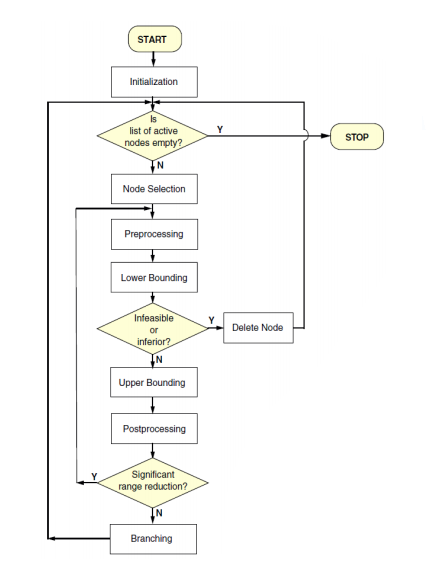
\includegraphics[width=85mm]{Algorithm_BARON.PNG}
\caption{BARON Algorithm \cite{Lipp2011BARONCME334}}
\label{fig_BARON}
\end{figure}

To solve the subproblems, BARON calls upon other solvers. By default, BARON utilizes CPLEX for linear problems and MINOS for nonlinear problems. CPLEX generally solves linear problems using the dual simplex algorithm. For problems with a nonlinear objective MINOS solves for local optima using a reduced gradient algorithm combined with a quasi-Newton algorithm. For problems with nonlinear constraints MINOS solves for local optima by using a projected Lagrangian algorithm. The program iterates through subproblems with linearized versions of the constraints and utilizes the reduced-gradient algorithm to solve \cite{GAMS_old}. 
\section{Aircraft Routing and Resources}
In \cite{Reiman2014} Reiman developed regression equations on flight data from aircraft performance manuals to estimate the fuel consumption required of the C-5, C-17, or the C-130 to climb, cruise and descend based on the aircraft gross weight, altitude and distance to travel. 
These mathematical models, in addition to a nodal reduction heuristic, were utilized to generate fuel efficient route alternatives for the strategic airlift problem. Follow-on research \cite{maywald} showed that fuel efficiency and cargo throughput can be improved using this alternative route method and the concept of hopping, compared to current cargo routes. Hopping is when an aircraft makes enroute stops to refuel thus allowing aircraft to carry more in payload weight instead of fuel weight to get to the destination \cite{Nangia2006OperationsRefuelling}. Extra stops require time, resource availability at enroute airfields of crews and aircraft maintenance, and the premise of hopping relies upon capitalizing on the fuel efficiency of smaller aircraft. While Maywald \textit{et. al.} \cite{maywald} do not account for resource availability, Baker \textit{et. al.} \cite{Baker2002OptimizingAirlift} evaluated the requirements for airfield resources to meet aircraft demand, including aircraft specific maintenance, ramp space and fuel pumping rates. 